\chapter{焦点面検出器アライメントの較正}
\label{chapter4}

GroundBIRD実験での偏光測定のためには、検出器間での信号の差分を取ることが重要であり、それに伴って望遠鏡のスキャンに対して最適な検出器のアライメントが求められる。この章では検出器アライメントの最適化に向けた改善を行い、観測データからその効果を確認した。

\section{検出器アライメントの問題点}

\subsection{スキャン軸に対する傾きと差分解析}
まず、GroundBIRDでの解析手法の1つである差分解析と検出器アライメントの関係について述べる。\ref{mkid_design}で示したように、焦点面検出器は異なる偏光方向に感度を持った検出器が交互に配置されている。これらの検出器が検出する信号は空のある点からの放射が望遠鏡内の光学系を経て焦点面へと届いたものである。つまり、焦点面での検出器の配置を空へと射影した時にどう配置されているかが重要になる。各検出器は空のある点を見ており、望遠鏡の方位角回転に伴って同じ仰角の空を回転しながら観測する(図\ref{scan_image})。
\begin{figure}[htbp]
  \centering
  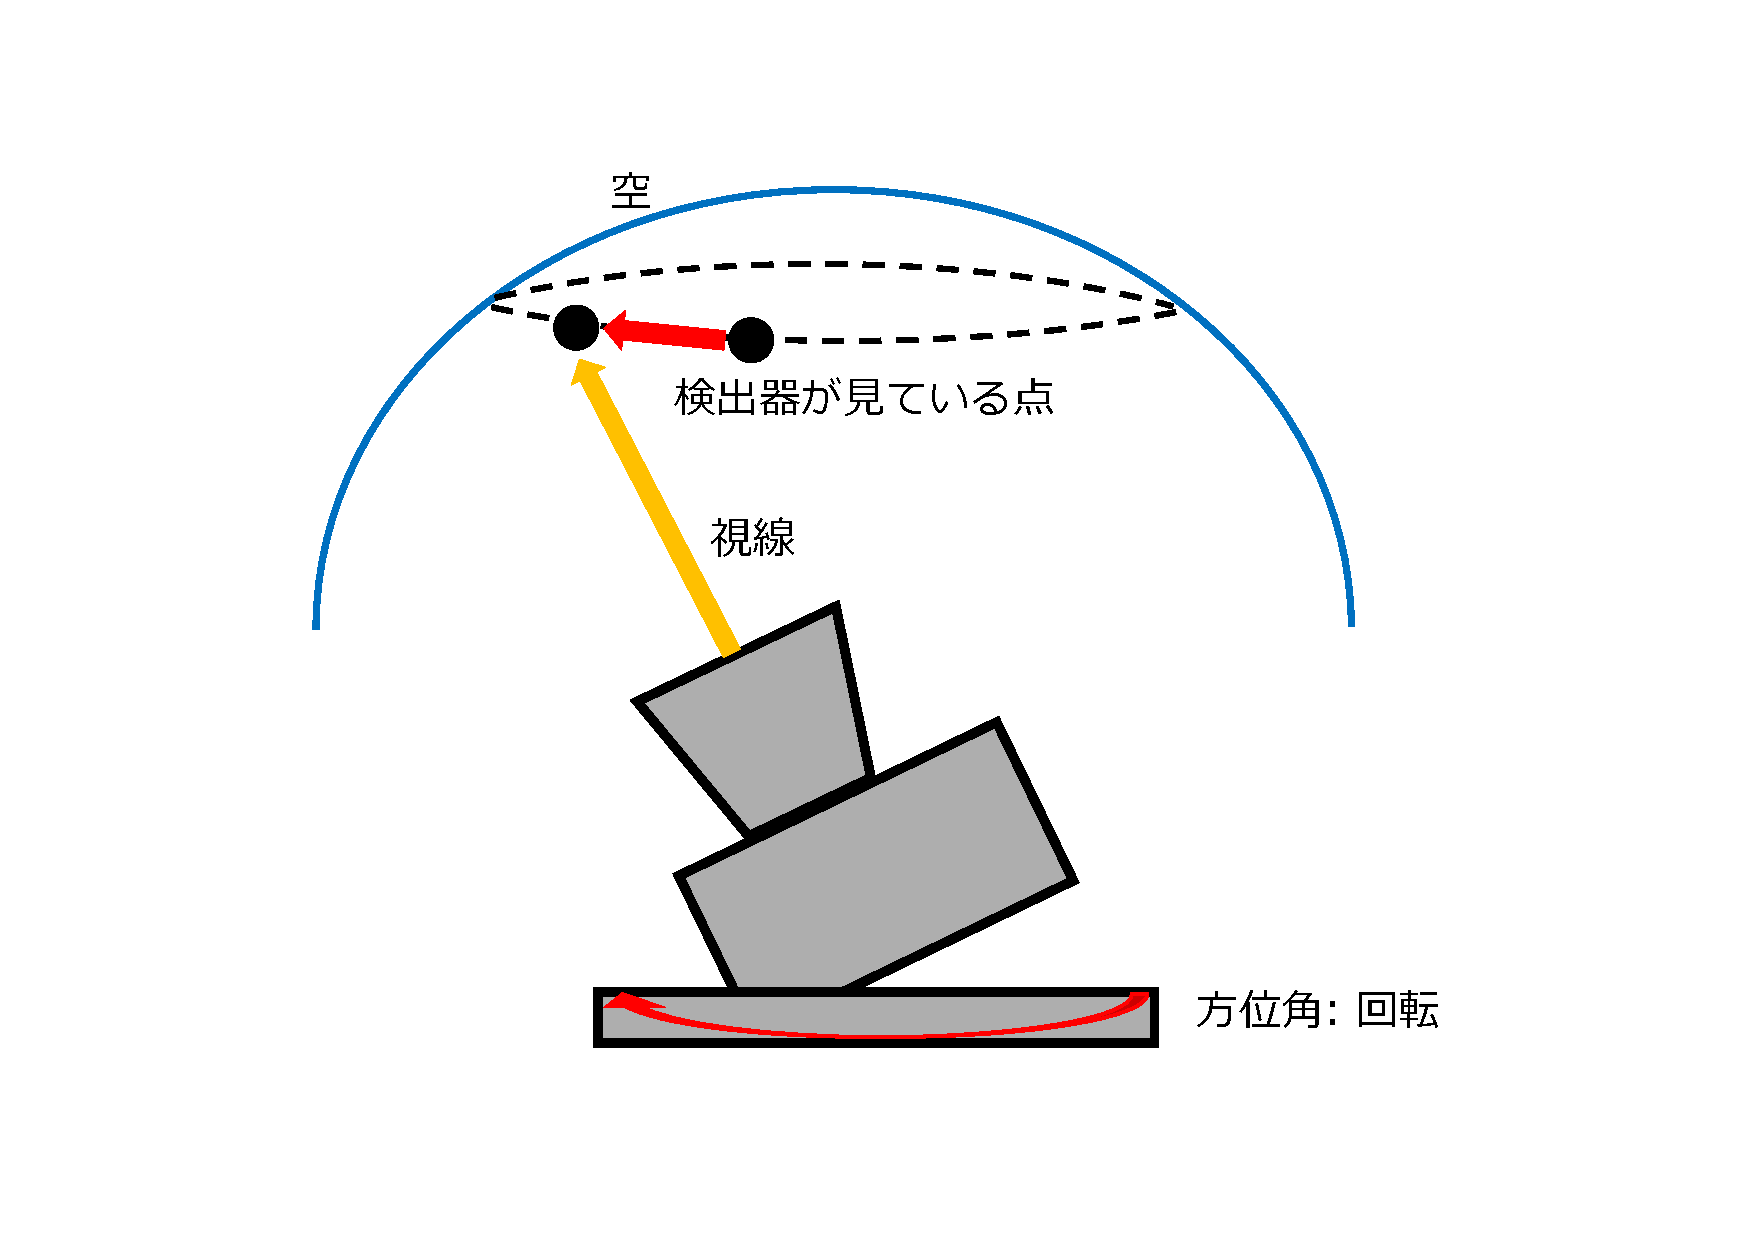
\includegraphics[width=0.6\columnwidth]{5_alignment/figs/scan_image.pdf}
  \caption{検出器が空の領域をスキャンする概要図。ある仰角を高速回転しながらスキャンする。}
  \label{scan_image}
\end{figure}
検出器で観測する信号は大きく(CMB + ノイズ)に分けられる。さらにノイズの中でも寄与が大きい成分に大気放射に由来するノイズがある。このノイズは刻一刻と変動する上に空の領域によっても異なっているため、高速回転によるスキャンで異なる検出器が同じ空の領域をスキャンすることで抑制できる。具体的には、異なる偏光方向に感度のある検出器が同じ仰角の空をスキャンする時、もう一方の検出器は片方の検出器が観測した空の領域をわずかな時間差で観測することができる。つまり、スキャンの間に大気の情報は変動せず観測される大気由来のノイズも変動しないことになる。そのため、検出器間で信号の差分をとることで、大気ノイズは共通していると考えれば取り除くことができ、偏光成分のみを残すことができる。しかし、検出器の配置がずれていて検出器間でスキャンする空の領域が異なる場合、大気の情報も異なり、差分をとっても大気ノイズを取り除くことができない(図\ref{scan_axis})。
\begin{figure}[htbp]
  \centering
  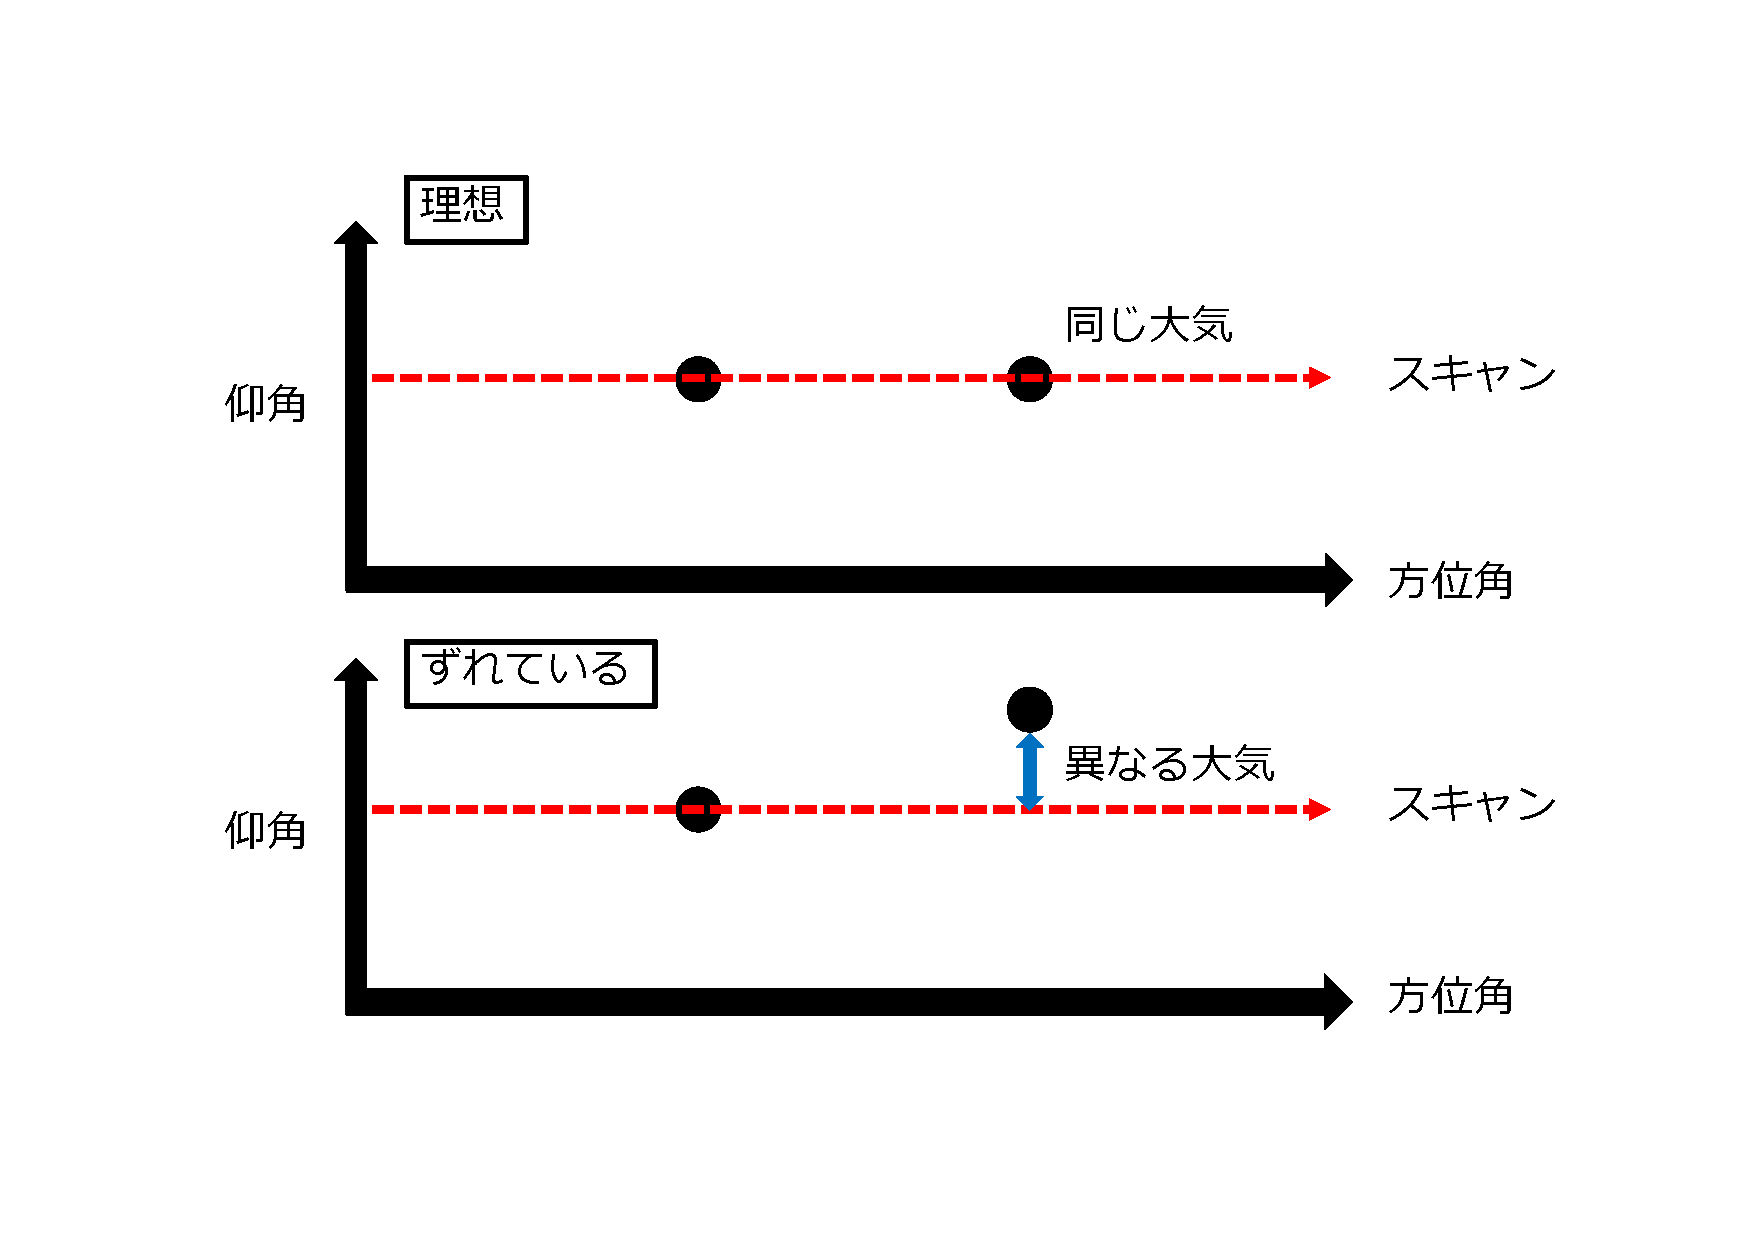
\includegraphics[width=0.7\columnwidth]{5_alignment/figs/scan_axis.pdf}
  \caption{空での理想的な検出器の配置とずれている場合の配置との比較。スキャン軸(方位角軸)に沿って検出器が並んでいないと観測する大気が検出器ごとに異なる。}
  \label{scan_axis}
\end{figure}

以上から空での理想的な検出器の配置は``複数の検出器がスキャン軸に沿って並んでいる''ことである。

しかし、観測データから理想的な検出器の配置からずれていることが示唆されていた。また、そのずれはスキャン軸に対して無視できないほどに有意な角度で傾いているものだと考えられていたが十分な検証と較正(実際に何度傾いているのか、傾きがあることでどれ程大気ノイズの影響が残ってしまうのか、など)がされていなかった。検出器アライメントの問題を改善し、GroundBIRDが持つ観測性能を最大限に引き出すことは質の良いデータを取得するためには不可欠である。

\subsection{要求される理想的なアライメント}

GroundBIRDにおける理想的な検出器の配置について詳細を見ていく。焦点面検出器は図\ref{full_array_picture}のように7つの検出器アレイが平面的に取り付けられているが、この検出器が観測する領域は平面のまま空に射影される訳ではない。観測する空の点は天球面上に張り付いた点と考えられるため、球面として射影される。焦点面検出器が平面を見るときと空を見る時での理想的な配置の違いを図\ref{distortion_pos}に示す。実際には球面から来る歪みの影響を受けた配置として空を観測することになり、望遠鏡の視線中心(\SI{220}{GHz}アレイ)ではほぼ平面だが、中心から離れた検出器は歪みの影響が出る。歪みを考慮した上で複数の検出器をスキャン軸に沿って並べることは焦点面の設計上難しい。また、高周波になるほど大気放射の寄与が大きくなる\cite{atmos_radiation}ことから、本論文では歪みの影響が少なく、大気放射の寄与も大きい中心の\SI{220}{GHz}アレイに対して配置がスキャン軸に沿って並んでいることを理想的なアライメントとする。
\begin{figure}[htbp]
  \centering
  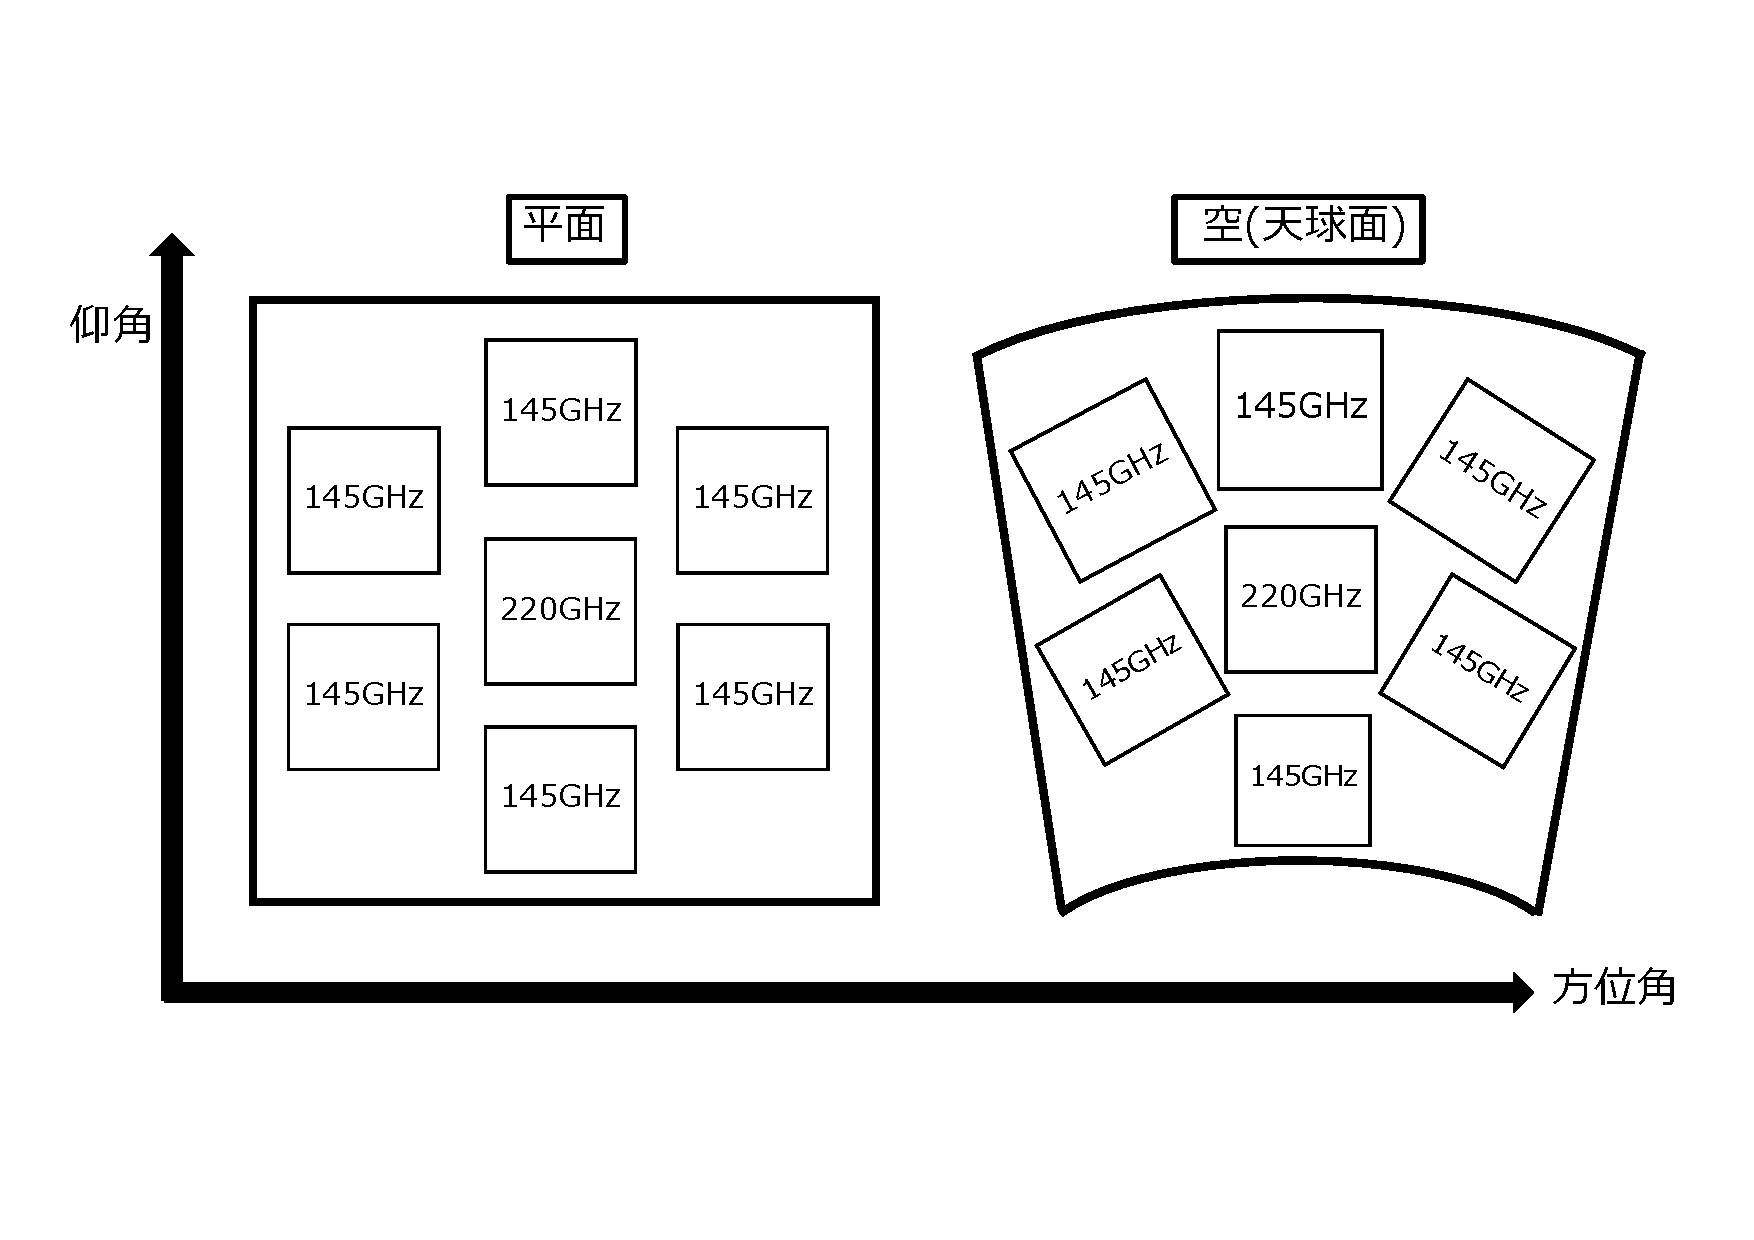
\includegraphics[width=0.8\columnwidth]{5_alignment/figs/distortion_pos2.pdf}
  \caption{平面と空(天球面)での理想的な検出器配置の違い。}
  \label{distortion_pos}
\end{figure}
\subsection{視線軸方向まわりの回転による較正}

スキャン軸に対して傾いた焦点面検出器を理想とする配置にするためには、検出器の視線を回転させてスキャン軸に並べれば良いことになる。また、焦点面検出器は望遠鏡内部で固定されているため望遠鏡全体の視線を回転することに対応する。つまり、望遠鏡のビーム中心を望遠鏡の視線方向とし、視線方向軸周りに適当な角度回転させることで各検出器の視線を回転させる(図\ref{boresight_axis})。
\begin{figure}[htbp]
  \centering
  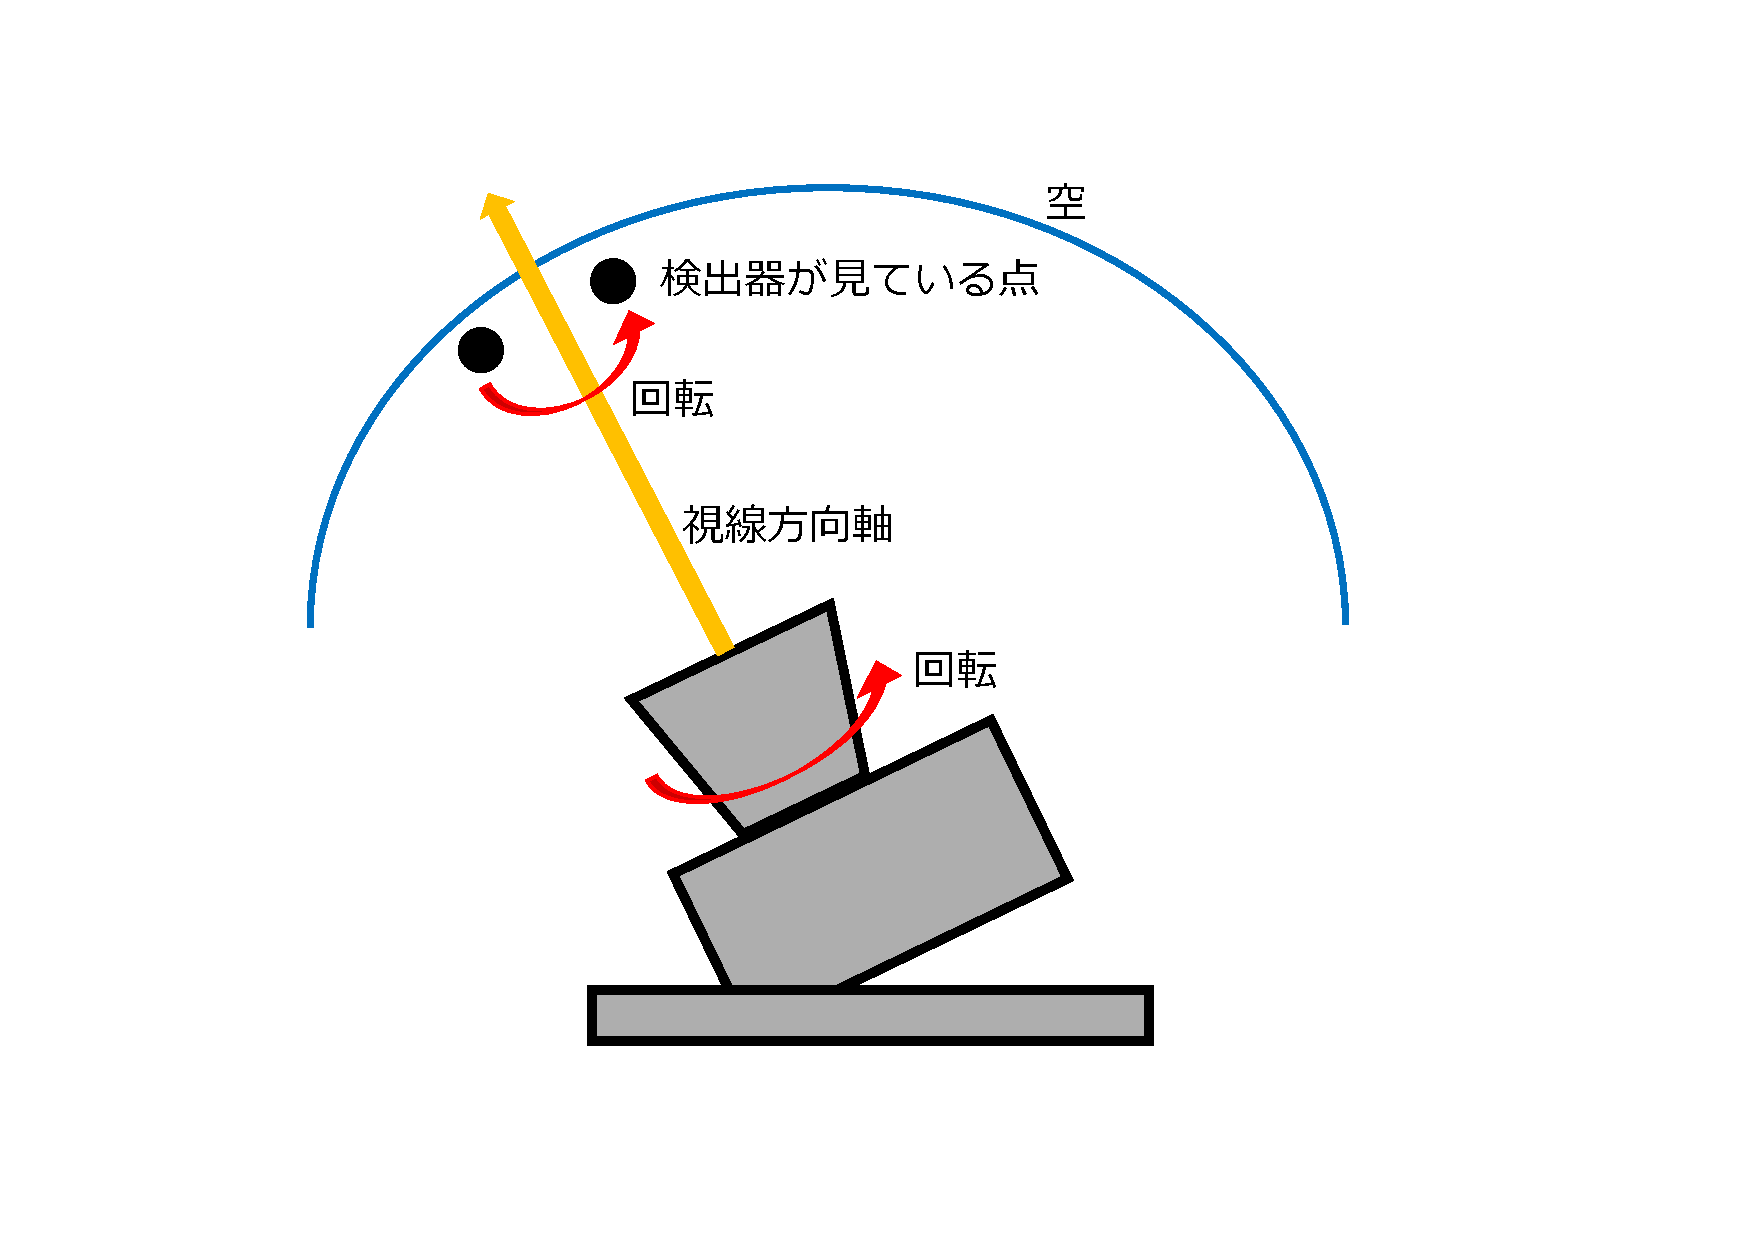
\includegraphics[width=0.8\columnwidth]{5_alignment/figs/boresight_axis.pdf}
  \caption{望遠鏡の視線方向軸と軸周りの回転。検出器の見ている点(視線)も回転する。}
  \label{boresight_axis}
\end{figure}
%検出器の配置がビームの中心に対して傾いている場合、視線方向軸の周りに望遠鏡を適当な角度回転させることで配置をスキャン軸に沿って並ばせることが可能になる。

そのため、理想的なアライメントにするための回転角を見積もる必要がある。回転角を求めるには各検出器の見ている点を知る必要があり、天体の観測データを解析することで算出できる(天体の運動が分かっているので検出器データと角度データから各検出器の視線情報を求められる)。

\section{月を用いた回転角の算出}

\subsection{月を用いた理由}

GroundBIRDで観測できる天体として月や惑星(木星、金星)が挙げられる。しかし、月と惑星ではデータの性質は大きく異なり、それぞれ観測上の長所と短所が存在する。月データと惑星データの特徴を表\ref{moon_vs_planet}に示す。
\begin{table}[htbp]
  \centering
  \caption{月データと惑星データの比較\cite{sueno_doctor}}
  \vspace{3mm}
  \begin{tabular}{ccc} \hline
    & 月 & 惑星 \\ \hline
    長所 &
    \begin{tabular}{c}
    S/N比が高い \\ (1度の観測で十分な信号を得られる)
    \end{tabular} &
    \begin{tabular}{c}
    点源として扱える \\ (視野角がビーム幅に比べて十分小さい)
    \end{tabular} \\ \hline
    短所 &
    \begin{tabular}{c}
    点源として扱えない \\ (輝度温度の非一様性が生じる)
    \end{tabular} &
    \begin{tabular}{c}
    S/N比が小さい \\ (データを蓄積しないとノイズに埋もれる)
    \end{tabular} \\ \hline
  \end{tabular}
  \label{moon_vs_planet}
\end{table}
検出器の視線情報を得るには点源として扱え、正確に点として求められる惑星が適しているが、\ref{jupiter_ana}で見るように点源で最も明るい木星の観測データでもノイズの影響をかなり受けてしまう。そのため、データを蓄積するか、PWVや湿度が十分低く観測条件が整った観測データを使用する必要がある。一方、月は高いS/N比により1度の観測データで十分な信号を得られ、データを蓄積することによるノイズが加わることなく解析ができる。点源として扱えないことによる誤差はあるものの、高いS/N比がそれをカバーできると考えたため、月のデータを選択した。

\subsection{必要な回転角}

\subsection{回転する上でのジグの必要性}

\section{ジグの設計と現地インストール}

\subsection{固定用ジグの作成}

\subsection{望遠鏡への実装}

\section{天体を用いた較正結果の確認}

\subsection{月データによる確認}

\subsection{木星データによる確認}
\label{jupiter_ana}

\section{検出器間差分で見る大気揺らぎの抑制}

\subsection{timing offsetの算出}

\subsection{差分解析による確認}
